%%%%%%%%%%%%%%%%%%%%%%%%%%%%%%%%%%%%%%%%%
% Beamer Presentation
% LaTeX Template
% Version 1.0 (10/11/12)
%
% This template has been downloaded from:
% http://www.LaTeXTemplates.com
%
% License:
% CC BY-NC-SA 3.0 (http://creativecommons.org/licenses/by-nc-sa/3.0/)
%
% Modified by Jeremie Gillet in November 2015 to make an OIST Skill Pill template
%
%%%%%%%%%%%%%%%%%%%%%%%%%%%%%%%%%%%%%%%%%

%----------------------------------------------------------------------------------------
%	PACKAGES AND THEMES
%----------------------------------------------------------------------------------------

\documentclass{beamer}

\mode<presentation> {

\usetheme{Madrid}

\definecolor{OISTcolor}{rgb}{0.65,0.16,0.16}
\usecolortheme[named=OISTcolor]{structure}

%\setbeamertemplate{footline} % To remove the footer line in all slides uncomment this line
%\setbeamertemplate{footline}[page number] % To replace the footer line in all slides with a simple slide count uncomment this line

\setbeamertemplate{navigation symbols}{} % To remove the navigation symbols from the bottom of all slides uncomment this line
}

\usepackage{graphicx} % Allows including images
\usepackage{booktabs} % Allows the use of \toprule, \midrule and \bottomrule in tables
\usepackage{textpos} % Use for positioning the Skill Pill logo
\usepackage{fancyvrb}
\usepackage{tikz}
\usepackage{hyperref}
\usepackage{listings}

\definecolor{dkgreen}{rgb}{0,0.6,0}
\definecolor{gray}{rgb}{0.5,0.5,0.5}
\definecolor{mauve}{rgb}{0.58,0,0.82}

\lstset{frame=tb,
  language=python,
  aboveskip=3mm,
  belowskip=3mm,
  showstringspaces=false,
  columns=flexible,
  basicstyle={\small\ttfamily},
  numbers=none,
  numberstyle=\tiny\color{gray},
  keywordstyle=\color{blue},
  commentstyle=\color{dkgreen},
  stringstyle=\color{mauve},
  breaklines=true,
  breakatwhitespace=true,
  tabsize=3
}

%----------------------------------------------------------------------------------------
%	TITLE PAGE
%----------------------------------------------------------------------------------------

\title[Skill Pill]{Skill Pill: Julia} % The short title appears at the bottom of every slide, the full title is only on the title page
\subtitle{Lecture 1: Introduction}

\author{Ankur Dhar \& James Schloss} % Your name
\institute[OIST] % Your institution as it will appear on the bottom of every slide, may be shorthand to save space
{
\textit{ankurd@oist.jp} \\ % Your institution for the title page
\textit{james.schloss@oist.jp} % Your email address
}
\date{July 11, 2019} % Date, can be changed to a custom date

\begin{document}

\setbeamertemplate{background}{
\includegraphics[width=\paperwidth]{SPbackground.png}} % Adding the background logo

\begin{frame}
\vspace*{1.4cm}
\titlepage % Print the title page as the first slide
\end{frame}

\setbeamertemplate{background}{} % No background logo after title frame

\addtobeamertemplate{frametitle}{}{% Adding the Skill Pill logo on the title screen after title frame
\begin{textblock*}{100mm}(.92\textwidth,-0.9cm)

\includegraphics[height=0.85cm]{julia.pdf}
\end{textblock*}}

\begin{frame}
  \tableofcontents
\end{frame}
\section{Introduction}



\subsection{Why does Julia exist}
\begin{frame}{Why does Julia exist?}
%  \pause
  \begin{block}{Key Points}
    \begin{enumerate}
    	   	
      \item Low-level languages are fast, but high level languages are readable.
      \item Recent advances in compiler design could bridge these two aspects.
      \item Julia is being openly developed by researchers, for researchers.
    \end{enumerate}
  \end{block}
%\pause
  The old mission statement is available \href{https://julialang.org/blog/2012/02/why-we-created-julia}{\color{blue} here} and some good discussion is available at \href{https://discourse.julialang.org/t/julia-motivation-why-werent-numpy-scipy-numba-good-enough/2236/}{\color{blue} here}. 
%\pause
  \begin{block}{My personal reason}
    A fast, open-source, high level language that is powerful enough to do serious numerical work, while being designed to encourage good code.
  \end{block}

\end{frame}
\subsection{What is wrong with the status quo}
\begin{frame}{The other contenders}
  The typical languages used in science are
  \begin{enumerate}
    \item Python
    \item Matlab
    \item R
  \end{enumerate}

  Once a problem is becoming to big we usually move to
  \begin{enumerate}
    \item C/C++
    \item Fortran
  \end{enumerate}
  This is called the 2+ language problem and Julia is trying to solve that.
\end{frame}

\begin{frame}{Python and Numpy}
  \begin{itemize}
    \item The compilers that exist (Numba) only work on primitive types and not user defined ones.
    \item GIL (Global Interpreter Lock) mask multi-threading hard.
    \item For fast code you need to write it in C.
    \item Numpy is great, but awful syntax for math.
  \end{itemize}
\end{frame}

\begin{frame}{Matlab}
  \begin{itemize}
    \item It costs a lot of money and is not open-source.
    \item Matlab will only be fast for a subset of operations.
    \item Matlab tends to hide the computer from the programmer.
  \end{itemize}
\end{frame}

\begin{frame}{A (biased) performance comparision}
  \center
  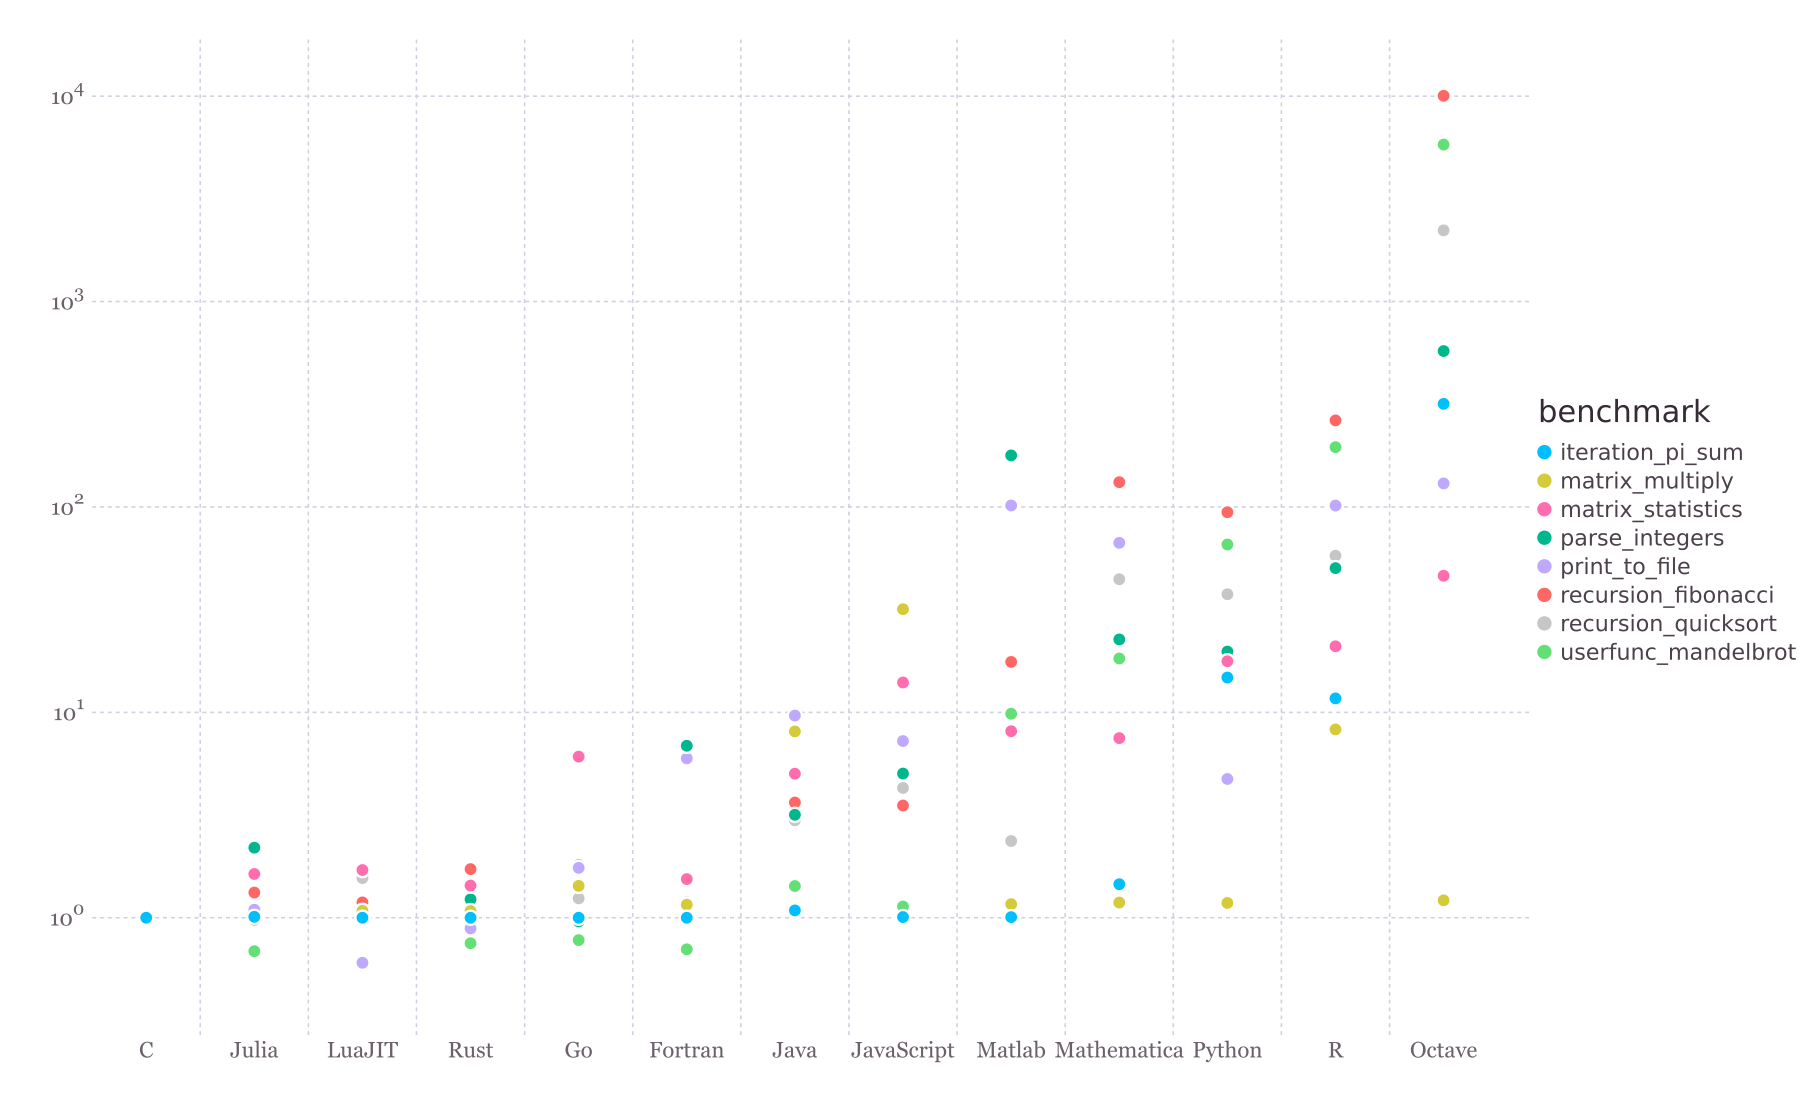
\includegraphics[width=\linewidth]{benchmarks}
\end{frame}

\section{Getting started}
\begin{frame}[fragile]{The REPL}
  \begin{block}{The Read-Eval-Print-Loop}
    The REPL is a command-line interface to Julia and is ideal for short experiments.
    \begin{Verbatim}[fontsize=\footnotesize]
               _
   _       _ _(_)_     |  Documentation: https://docs.julialang.org
  (_)     | (_) (_)    |
   _ _   _| |_  __ _   |  Type "?" for help, "]?" for Pkg help.
  | | | | | | |/ _` |  |
  | | |_| | | | (_| |  |  Version 1.1.1 (2019-05-16)
 _/ |\__'_|_|_|\__'_|  |  Official https://julialang.org/ release
|__/                   |

julia> 

\end{Verbatim}

In the \verb|REPL| you can use \verb|?| to switch your \verb|REPL| mode into help mode and get information about functions.
  \end{block}
\end{frame}
\begin{frame}{IDEs}
  There are two main IDEs that are \emph{feature} complete and can be used for Julia. The main one is based on Atom and is called Juno \url{http://junolab.org/}.

\vspace{0.5cm}
  The second one is based on on Visual Studio Code and available at \url{https://marketplace.visualstudio.com/items?itemName=julialang.language-julia}.

\vspace{0.5cm}
  We will not be using these during the course, but you are welcome to try them out
\end{frame}
\begin{frame}[fragile]{Jupyter}
  Jupyter is an interactive web-based client for Python, Julia, R and many other languages.
  It offers a programming environment that is well suited for explorative data analysis or prototyping.
  \begin{block}{Installation}
  \begin{Verbatim}
    julia> ENV["JUPYTER"] = ""
    julia> ] add IJulia
    \end{Verbatim}
  \end{block}
  \begin{block}{Starting a Jupyter session}
    \begin{Verbatim}
    julia> using IJulia
    julia> notebook()
    \end{Verbatim}
  \end{block}
  \begin{block}{JuliaBox}
    There is an online service provided by JuliaComputing at \url{https://juliabox.com} that gives you a cloud version of Jupyter.
  \end{block}
\end{frame}
\section{Language syntax and semantics}
\begin{frame}[fragile]{Variables and datatypes}
  Julia is a dynamic language and so you can simply create variables in any scope.
  \begin{lstlisting}
  x = 1   # x will be of type Int64
  y = 1.0 # y will be of type Float64
  z = 1.0 - 2.0im # z will be an Complex{Float64}
  1//2 # Rational numbers
  "This is a String"
  """
  This is a multiline
  String
  """
  'C' # Character literal
  1.0f0 # Float32 literal
  \end{lstlisting}
  Use \verb|typeof| to check the type of any variable. Variable names can be unicode and so greek symbols can be used.
  In the \verb|REPL| and most editors you can insert them by entering their \LaTeX name and press\verb|[Tab]|.
\end{frame}
\begin{frame}[fragile]{Conditionals}
  Julia has all the typical conditionals \verb|if|, \verb|else|, \verb|elseif| which have to end in an \verb|end|.
  Blocks in Julia are not whitespace sensitive and conditionals do not need to be wrapped in round brackets.

  \begin{lstlisting}
  if rand() < 0.5
    println("Hello there!")
  else
    println("Go away!")
  end
  \end{lstlisting}

\end{frame}
\begin{frame}[fragile]{Loops}
  Julia has \verb|for| and \verb|while| loops. A \verb|while| loop takes a condition and a \verb|for| loop takes a iteratior.
  One can use \verb|break| to break out of a loop and \verb|continue| to skip to the next iteration. It is noteworthy that a \verb|for| loop can take an arbitrary iterator and even desugar tuples.
  \begin{lstlisting}
  for (i, x) in enumerate(['A', 'B', 'C'])
    if x == 'B'
      continue
    end
    println(i)
  end

  while true
    # ternary operator ?!
    rand() < 0.1 ? break : println("You are trapped!")
  end
  \end{lstlisting}
\end{frame}
\begin{frame}[fragile]{Functions and lambdas}
  Julia uses functions to organize operations. Every function is compiled for the combination of input parameters.
  \begin{lstlisting}
  """
      f(x, y)

  `f` will add two numbers together.
  """
  function f(x, y)
    return x + y
  end

  g(x) = x^2

  h = (x)-> 1/x
  map(lowercase, ['A', 'B', 'C'])
  map((x)->x+2, [1, 2, 3])
  \end{lstlisting}
\end{frame}
\begin{frame}[fragile]{Types}
  Julia's type system allows you to restrict functions to certain types and specialized functions for others.
  You can also create your own types. The names of types are typically captialized while functions are lowercase.
  \begin{lstlisting}
  abstract type Entity end
  mutable struct Player <: Entity 
    mass::Float64
    name::String
    position::Tuple{Float64, Float64}
  end
  struct Object <: Entity
    position::Tuple{Float64, Float64}
  end
  newObject=Object(0,0)
  \end{lstlisting}
\end{frame}
\begin{frame}[fragile]{Multiple dispatch in a nutshell}
  Julia is not an Object-Oriented programming language so functions do not belong to an object.
  A function is a set of multiple methods each with their own signatures. When you call a function the most specific methods is executed.

  \begin{lstlisting}
  function h(x::Number)
    println("x is most definitly a number.")
  end
  function h(x::Integer)
    println("x is a integer")
  end
  function h(x::Int8)
    println("Specific method for Int8")
  end
  \end{lstlisting}
  This becomes really powerful when having multiple argurments and being able to select the most specific method.
\end{frame}
\begin{frame}[fragile]{Modules}
  Julia code is organised as modules (namespaces). Module names are capitalised and you can nest modules as well.

  \begin{lstlisting}
  module MyModule
    export f

    g() = "Internal function"
    f() = println(g())
  end
  using Main.MyModule
  \end{lstlisting}
\end{frame}
\section{The ecosystem}
\begin{frame}[fragile]{Installing packages}
  Julia has an inbuilt package manager called \verb|Pkg|. You can access it from the REPL by entering \verb|]|. Julia packages end in \verb|.jl|
  and it is customary to refer to them by their full name online, but within Julia you drop the \verb|.jl|.
  So to install the Julia package \verb|Distributions.jl| in the \verb|REPL| just run:

  \begin{lstlisting}
  ] add Distributions
  \end{lstlisting}

  A few other commands:
  \begin{lstlisting}
  # Updating the installed packages
  ] update
  # What packages are installed?
  ] status
  \end{lstlisting}
  In order to create your own packages you have to install \verb|PkgDev.jl|.
\end{frame}
\begin{frame}{Resources}
\begin{description}
	\item[Documentation] \url{https://docs.julialang.org/en/v1.1/}
	\item[Forum] \url{https://discourse.julialang.org}
	\item[Issue Tracker] \url{https://github.com/JuliaLang/julia}
	\item[Downloads] \url{https://julialang.org/downloads/}
	\item[Packages] \url{https://pkg.julialang.org/}
	\item \url{https://juliaobserver.com/}
\end{description}
\end{frame}
\begin{frame}{What is next?}
  \begin{block}{Question?!}
    What do you want to hear learn about?
  \end{block}
  \begin{description}
    \item[Next Session] How to use Julia for computation and plotting
    \item[Next Tuesday] Data Structures and Algorithms.
  \end{description}
\end{frame}

\end{document}
